%Copyright 2019 Christopher M. Jermaine (cmj4@rice.edu) and Risa B. Myers (rbm2@rice.edu)
%
%Licensed under the Apache License, Version 2.0 (the "License");
%you may not use this file except in compliance with the License.
%You may obtain a copy of the License at
%
%    https://www.apache.org/licenses/LICENSE-2.0
%
%Unless required by applicable law or agreed to in writing, software
%distributed under the License is distributed on an "AS IS" BASIS,
%WITHOUT WARRANTIES OR CONDITIONS OF ANY KIND, either express or implied.
%See the License for the specific language governing permissions and
%limitations under the License.
%===============================================================
\documentclass[aspectratio=169]{beamer}
\mode<presentation>
{
\usetheme[noshadow, minimal,numbers,riceb,nonav]{Rice}
\usefonttheme[onlymath]{serif}
\setbeamercovered{transparent}
}
\useinnertheme{rectangles}

\usepackage[english]{babel}

\usepackage{mathptmx}
\usepackage{helvet}
\usepackage{courier}
\usepackage[T1]{fontenc}
\usepackage{trajan}
\usepackage{ textcomp }
\usepackage{listings}

\newenvironment{noindentitemize}
{ \begin{itemize}
 \setlength{\itemsep}{1.5ex}
  \setlength{\parsep}{0pt}   
  \setlength{\parskip}{0pt}
 \addtolength{\leftskip}{-2em}
 }
{ \end{itemize} }

\newenvironment{noindentitemize2}
{ \begin{itemize}
  \setlength{\itemsep}{0ex}
  \setlength{\parskip}{0pt}
  \setlength{\parsep}{0pt}   
  \addtolength{\leftskip}{-2em}  }
{ \end{itemize} }



\lstnewenvironment{SQL}
  {\lstset{
        aboveskip=5pt,
        belowskip=5pt,
        escapechar=!,
        mathescape=true,
        upquote=true,
        language=SQL,
        basicstyle=\linespread{0.94}\ttfamily\footnotesize,
        morekeywords={PRINT, CURSOR, OPEN, FETCH, CLOSE, DECLARE, BEGIN, END, PROCEDURE, FOR, EACH, WITH, PARTITION, 	TEST, WHETHER, PROBABILITY, OUT,LOOP,IF,CONTINUE, HANDLER,CALL, FUNCTION, RETURNS, LANGUAGE,BODY,RETURN, REPLACE,plpgsql,
        RAISE, NOTICE,
        REPLACE, ROW, BEFORE, EXIT, TEXT, REFCURSOR, QUOTE_LITERAL, DELIMITER,CONCAT,FOUND,LEAVE },
        deletekeywords={VALUE, PRIOR},
        showstringspaces=true}
        \vspace{0pt}%
        \noindent\minipage{0.65\textwidth}}
  {\endminipage\vspace{0pt}}
  
  
\lstnewenvironment{SQLtiny}
  {\lstset{
        aboveskip=5pt,
        belowskip=5pt,
        escapechar=!,
        mathescape=true,
        upquote=true,
        language=SQL,
        basicstyle=\linespread{0.94}\ttfamily\tiny,
        morekeywords={PRINT, CURSOR, OPEN, FETCH, CLOSE, DECLARE, BEGIN, END, PROCEDURE, FOR, EACH, WITH, PARTITION, 	TEST, WHETHER, PROBABILITY, OUT,LOOP,IF,CONTINUE, HANDLER,CALL, FUNCTION, RETURNS, LANGUAGE,BODY,RETURN, REPLACE,plpgsql,
        RAISE, NOTICE,
        REPLACE, ROW, BEFORE, EXIT, TEXT, REFCURSOR, QUOTE_LITERAL, DELIMITER,CONCAT,FOUND,LEAVE },
       deletekeywords={VALUE, PRIOR},
        showstringspaces=true}
        \vspace{0pt}%
        \noindent\minipage{0.47\textwidth}}
  {\endminipage\vspace{0pt}}

%===============================================================%

\title[]
{Tools \& Models for Data Science}

\subtitle{Introduction to Modeling 2}

\author[]{Chris Jermaine \& Risa Myers}
\institute
{
  Rice University 
}

\date[]{}

\subject{Beamer}


\begin{document}

\begin{frame}
 \titlepage
\end{frame}

%***********************************************************
\begin{frame}{Models Are Parameterized}

\begin{itemize}
\item Normal PDF: $\mu, \sigma$
\begin{itemize}
\item $\mu$ is the center of the distribution
\item $\sigma$ determines the width
\end{itemize}
$$f_{\textrm{Normal}}(x | \mu, \sigma) = \frac{1}{\sqrt{2\pi\sigma^2}}
                e^{-\frac{(x - \mu)^2}{2\sigma^{2}}}$$
%$$f_{\textrm{Normal}}(x | \mu, \sigma) = \sigma^{-1} (2\pi)^{-\frac{1}{2}}
%                e^{-\frac{1}{2}(x - \mu)^2\sigma^{-2}}$$
\item Exponential PDF: $\lambda$
$$f_{\textrm{Exp}} (x | \lambda) = \lambda e^{-\lambda x}$$
\item Key question: how to choose parameters?
\end{itemize}
\end{frame}
%***********************************************************
\begin{frame}{Models Are Parameterized}

\begin{itemize}
\item Normal PDF: $\mu, \sigma$
\begin{itemize}
\item $\mu$ is the center of the distribution
\item $\sigma$ determines the width
\end{itemize}
$$f_{\textrm{Normal}}(x | \mu, \sigma) = \frac{1}{\sqrt{2\pi\sigma^2}}
                e^{-\frac{(x - \mu)^2}{2\sigma^{2}}}$$
\item Exponential PDF: $\lambda$
$$f_{\textrm{Exp}} (x | \lambda) = \lambda e^{-\lambda x}$$
\item Key question: how to choose parameters?
\begin{itemize}
	\item Typically chosen to ``fit'' the model to example data
	\item To make the model a good explanation for the data
	\item Also called ``learning'' in ML
\end{itemize}
\end{itemize}

\end{frame}
%***********************************************************
\begin{frame}{Approaches to Learning a Model}

\begin{itemize}
\item There are many, including:
\begin{enumerate}
\item Optimization based (Least Squares)
\item Probabilistic: MLE (Maximum Likelihood Estimation)
\item Probabilistic: Bayesian
\item Deep Learning
\end{enumerate}
%\item We will cover the first 3
\end{itemize}
\end{frame}
%***********************************************************
\begin{frame}{Choosing an Approach to Learning a Model}

\begin{itemize}
\item Nature of the problem
\item Amount of data available
\item Tools available
\item Requirements of the model
\begin{itemize}
\item Interpretability
\item Availability
\item Familiarity
\item Experimentation
\item Accuracy
\end{itemize}
\end{itemize}
\end{frame}
%***********************************************************
\begin{frame}{Optimization-Based}

\begin{itemize}
\item Goal is to reduce some error metric on example/training data using a loss function
\begin{itemize}
\item Error tells us how well the model fits the TRAINING data
\end{itemize}
\item No direct probabilistic motivation
\item Common approach
\end{itemize}
\end{frame}
%***********************************************************
\begin{frame}{Lease Squares Regression}

\begin{itemize}
\item Goal: Minimize the sum of the squares of the residuals
\item[?] What is a residual?
\end{itemize}
\end{frame}
%***********************************************************
\begin{frame}{Lease Squares Regression}

\begin{itemize}
\item Goal: Minimize the sum of the squares of the residuals
\item What is a residual?
\begin{itemize}
\item Prediction error
\item The difference between the observed value and the model computed value

\end{itemize}
\item Compute the sum of the square of the residuals
\item [] $\sum_{i=1}^n r_i^2$
\item [] $\sum_{i=1}^n (f(t_i, \beta) - x_i)^2$ % switch order? rename x_i to y_i?
\item[] where $\beta$ is the set of model parameters and $x_i$ is the true outcome 
\end{itemize}
\end{frame}
%***********************************************************
\begin{frame}{Classic Example: Least Squares Regression}

\begin{columns}
\begin{column}{0.5\textwidth}
Example
\begin{itemize}
\item I observe $\langle 18, 22, 45, 49, 86\rangle$
\item At time ticks $\langle 1, 2, 3, 4, 5\rangle$
\item[?] How can I predict the next item?
\end{itemize}
\end{column}
\begin{column}{0.5\textwidth}
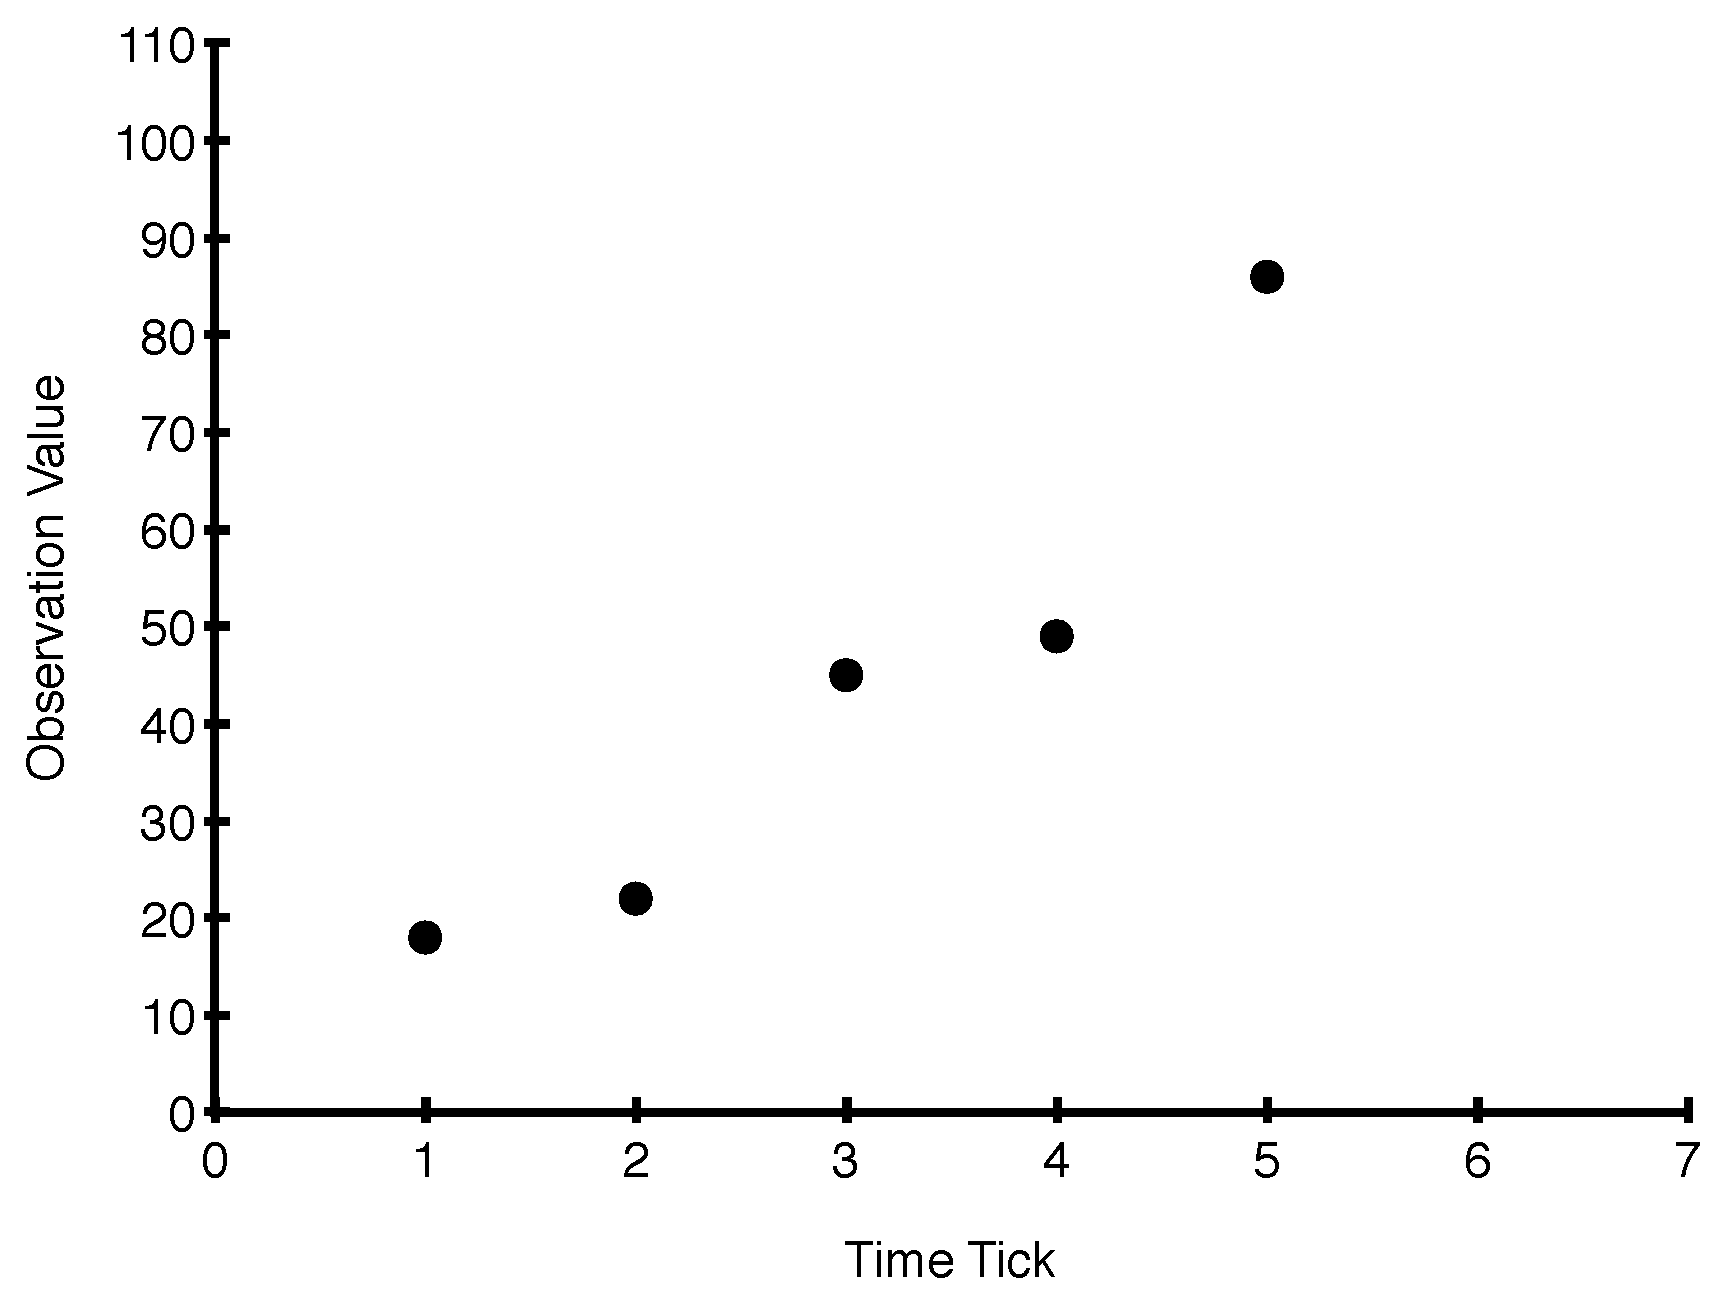
\includegraphics[width=1\textwidth]{lectModel2/LSReg1.pdf}
\end{column}
\end{columns}
\end{frame}
%***********************************************************
\begin{frame}{Example: Least Squares Regression}

\begin{columns}
\begin{column}{0.5\textwidth}
\begin{itemize}
\item I observe $\langle 18, 22, 45, 49, 86\rangle$
\item At time ticks $\langle 1, 2, 3, 4, 5\rangle$
\item How can I predict the next item?
\item $i$th observation is $x_i$, tick is $t_i$
	\begin{itemize}
		\item Might fit a line to the data
		\item So, $x_i \approx f(t_i) = m \times t_i$
		\item Where $m$ is the slope of the line
		\item Observation at time tick $i$ is a function of $t$
		\item $t_i$ is the $i$th time tick
		\item Here $t_i = i$ - our data is evenly spaced
	\end{itemize}
\end{itemize}
\end{column}
\begin{column}{0.5\textwidth}
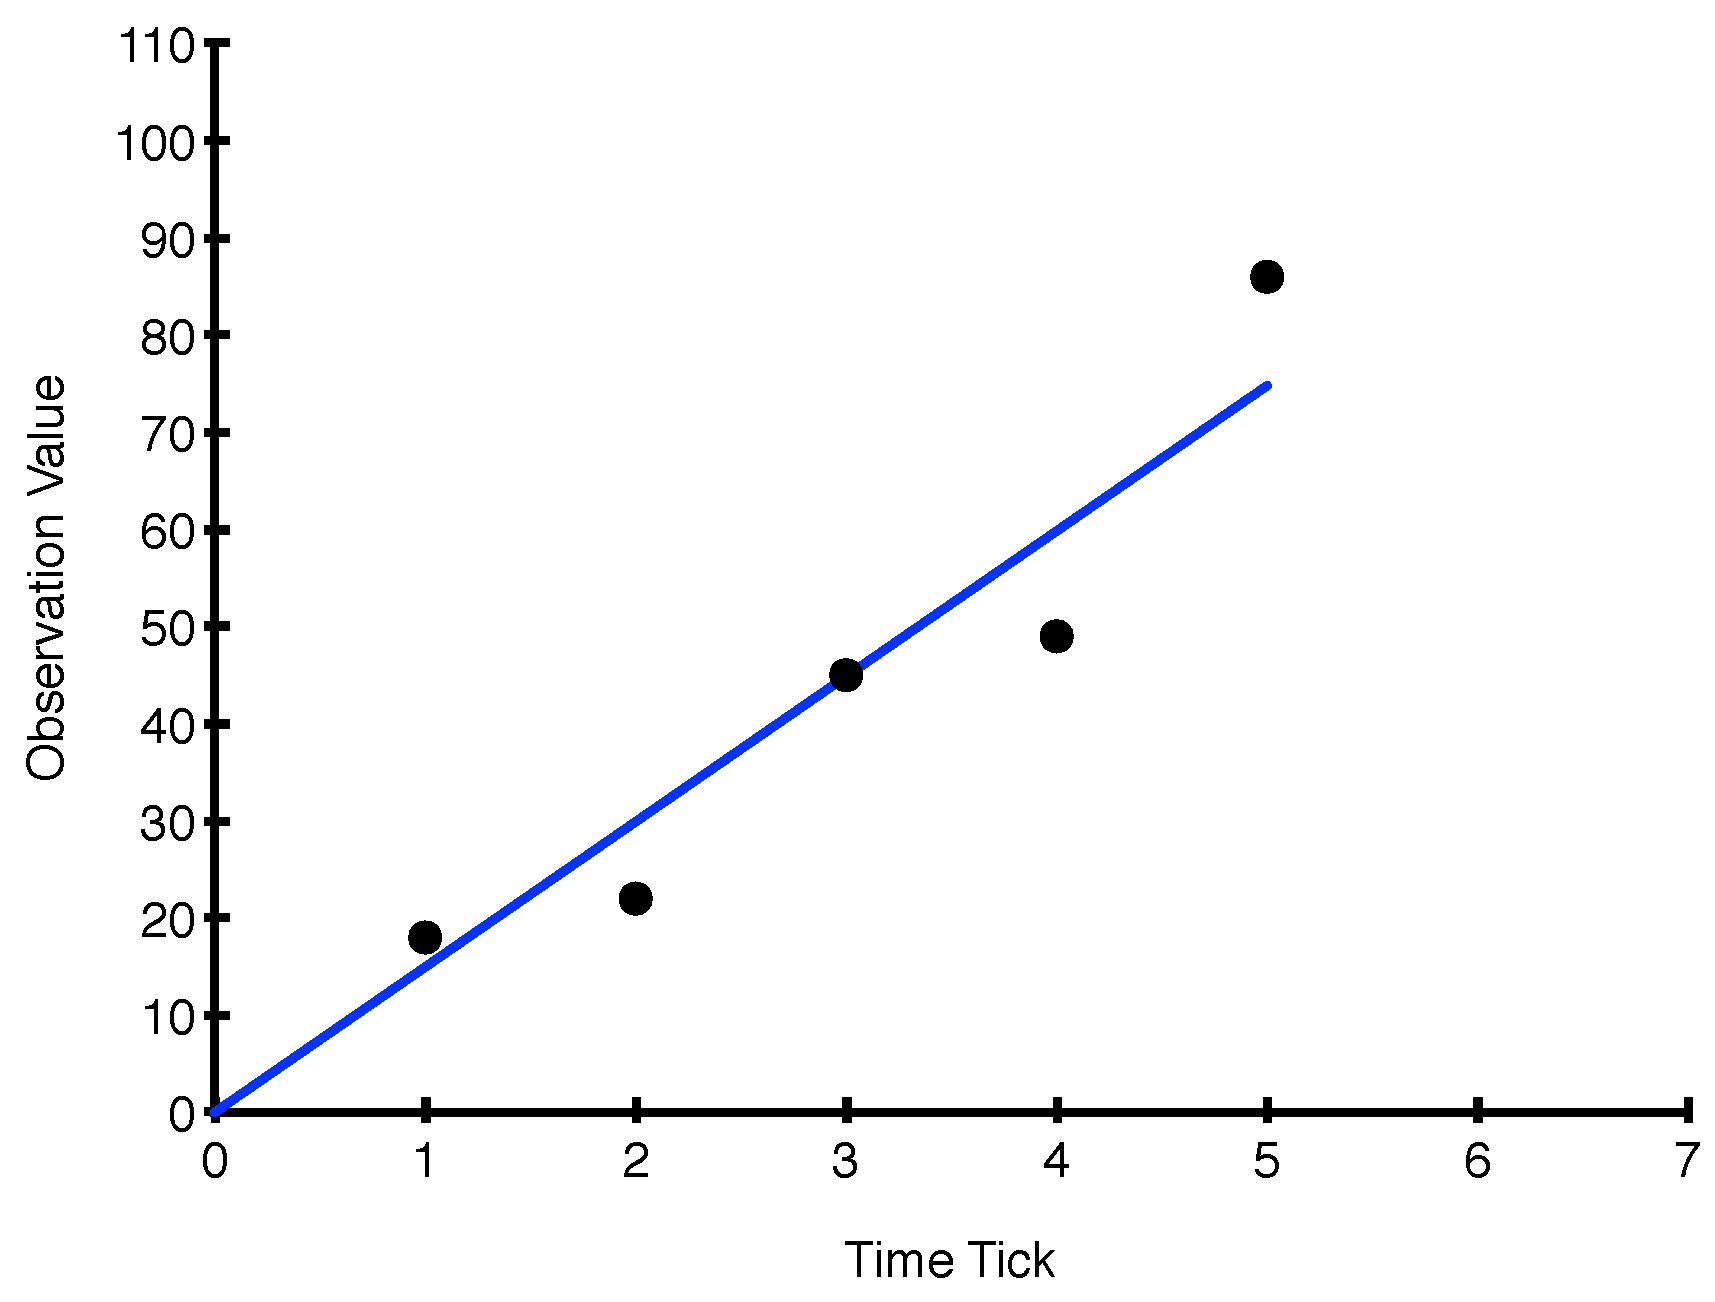
\includegraphics[width=1\textwidth]{lectModel2/LSReg1Line.pdf}
\end{column}
\end{columns}
\end{frame}
%***********************************************************
%\begin{frame}{Overlap of Approaches}
%\begin{itemize}
%\item Approaches may overlap
%\item Compare Least Squares to the PDF for the Normal distribution
%\begin{itemize}
%\item Includes a term with $e^{-\frac{(x - \mu)^2}{2\sigma^{2}}}$
%\item $(x - \mu)^2$ Looks a lot like Least Squares
%\end{itemize}
%\end{itemize}
%\end{frame}

%***********************************************************
\begin{frame}{Computing Least-Squares Fit}

	\begin{itemize}
		\item Loss function is the sum of the squares of the residuals
		\item This loss function is ``convex''
\end{itemize}
\end{frame}
%***********************************************************
\begin{frame}{What is a Convex Function?}


\begin{columns}
\begin{column}{0.7\textwidth}
\begin{itemize}
\item Intuition
\begin{itemize}
\item Continuous function 
\item The line connecting any two points is on or above the function
\item The function isn't ``wavy''
\item Strictly convex $\rightarrow$ 2nd derivative is always positive
\end{itemize}
%\item Formal definition
%\begin{itemize}
%\item 
%\end{itemize}
\item Examples
\begin{itemize}
\item Quadratic function $x^2$
\item Exponential function $e^x$
\end{itemize}

\item Benefits
\begin{itemize}
\item Strictly convex functions have at most one minimum
\item Differentiable
\end{itemize}
\end{itemize}
\end{column}
\begin{column}{0.3\textwidth}
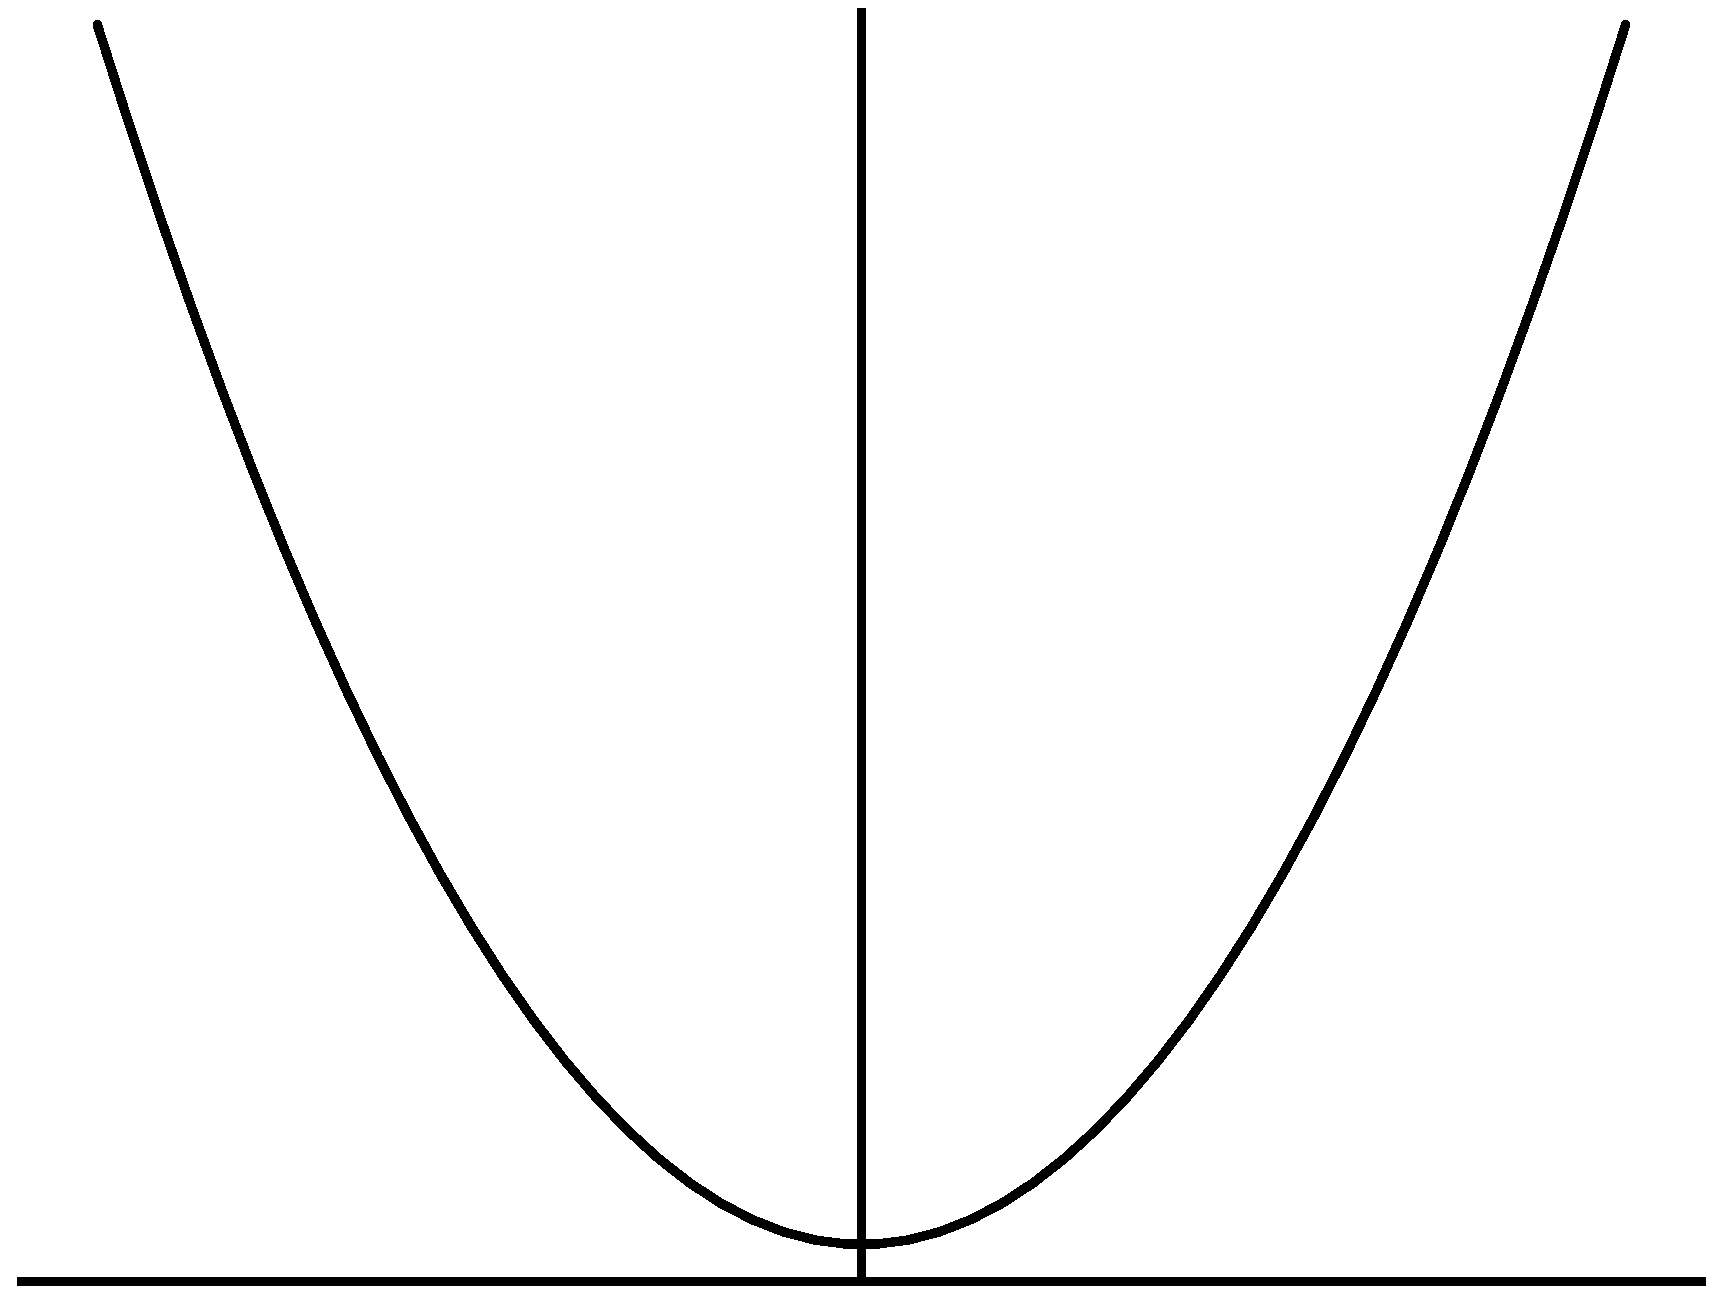
\includegraphics[width=.7\textwidth]{lectModel2/convex1.pdf}\\
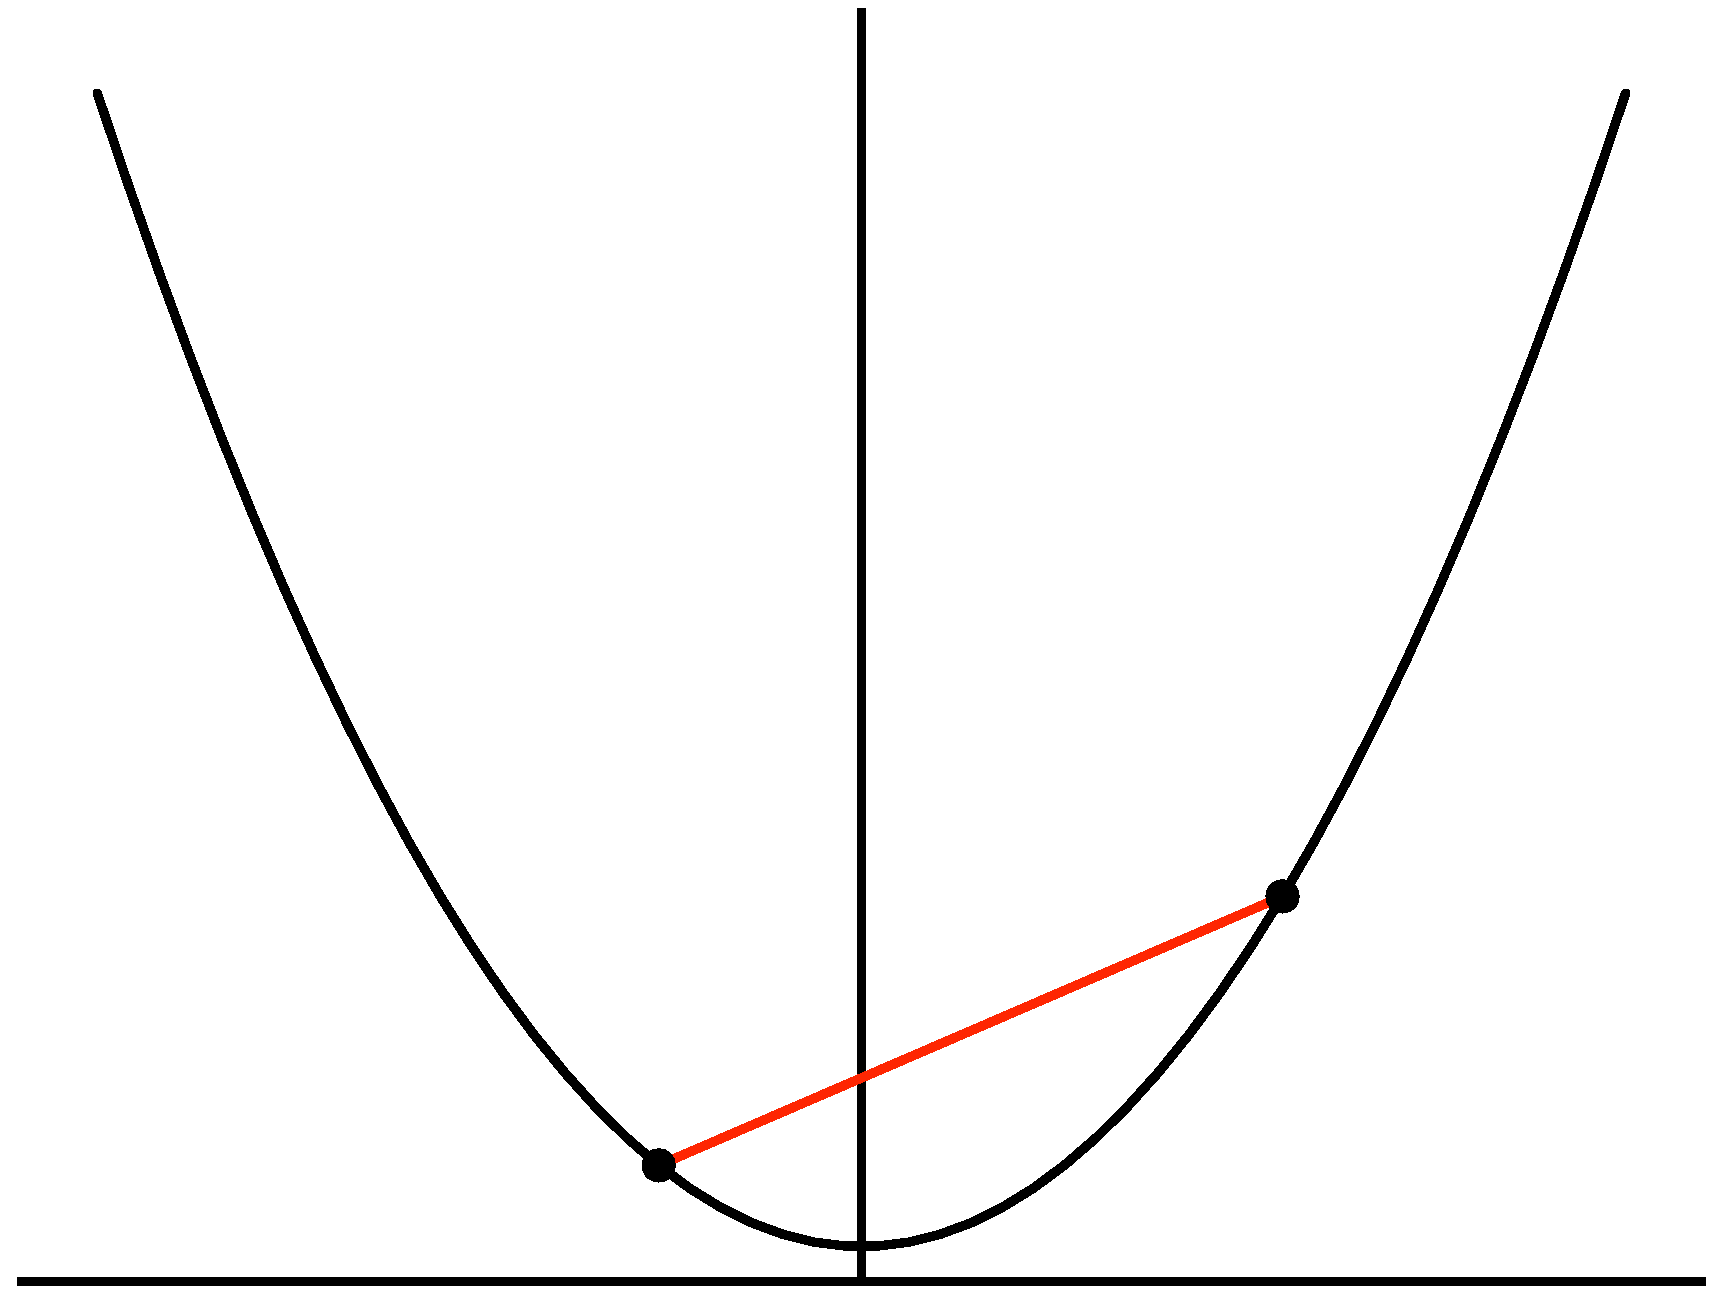
\includegraphics[width=.7\textwidth]{lectModel2/convex2.pdf}
\end{column}
\end{columns}

\end{frame}
%***********************************************************
\begin{frame}{Computing Least-Squares Fit}

	\begin{itemize}
		\item Choose unique $m$ where $l'(m) = 0$
		\item That is, where the derivative of the loss function = 0
		% locn of best answer for a convex function
\end{itemize}
\end{frame}
%***********************************************************
\begin{frame}{Computing Least-Squares Fit}
\begin{columns} [T]
\begin{column}{0.5\textwidth}
\begin{itemize}
\item[]
 \begin{align}
l(m) &= \sum_i \left(f(t_i) - x_i \right)^2 \nonumber \\
     &= \sum_i \left(m \times t_i - x_i \right)^2 \nonumber \\
l'(m) &= \sum_i 2t_i \left(m \times t_i - x_i \right) \nonumber  \\
      &= \sum_i 2mt_i^2 - 2t_ix_i \nonumber \\
      &= 2m(1 + 4 + 9 + 16 + 25) - 2(18 + 44 + 135 + 196 + 430) \nonumber \\
      &= 110m - 1646 \nonumber 
\end{align}
\item So loss minimized at $m = 14.96$
\item Recall $f(t_i) = m \times t_i$
\item[?] Value at time tick 6? %89.8
\end{itemize}
\end{column}
\begin{column}{0.5\textwidth}
\vspace{1.5em}
\begin{itemize}
\item Define loss function
\vspace{1em}
\item Sub in defn of $f$
\vspace{.5em}
\item Take the first derivative 
\item[] (chain rule)
%\vspace{1em}
\item Simplify
\vspace{.5em}
\item Plug in values
\item Solve for $m$
\end{itemize}
\end{column}
\end{columns}
\end{frame}

%***********************************************************
\begin{frame}{Next Value?}

\begin{columns} [T]
\begin{column}{0.5\textwidth}
\begin{itemize}
\item Recall $f(t_i) = m \times t_i$
\item Value at time tick 6? 
\item $f(6) = 14.96 \times 6 = 89.8$
\end{itemize}
\end{column}
\begin{column}{0.5\textwidth}
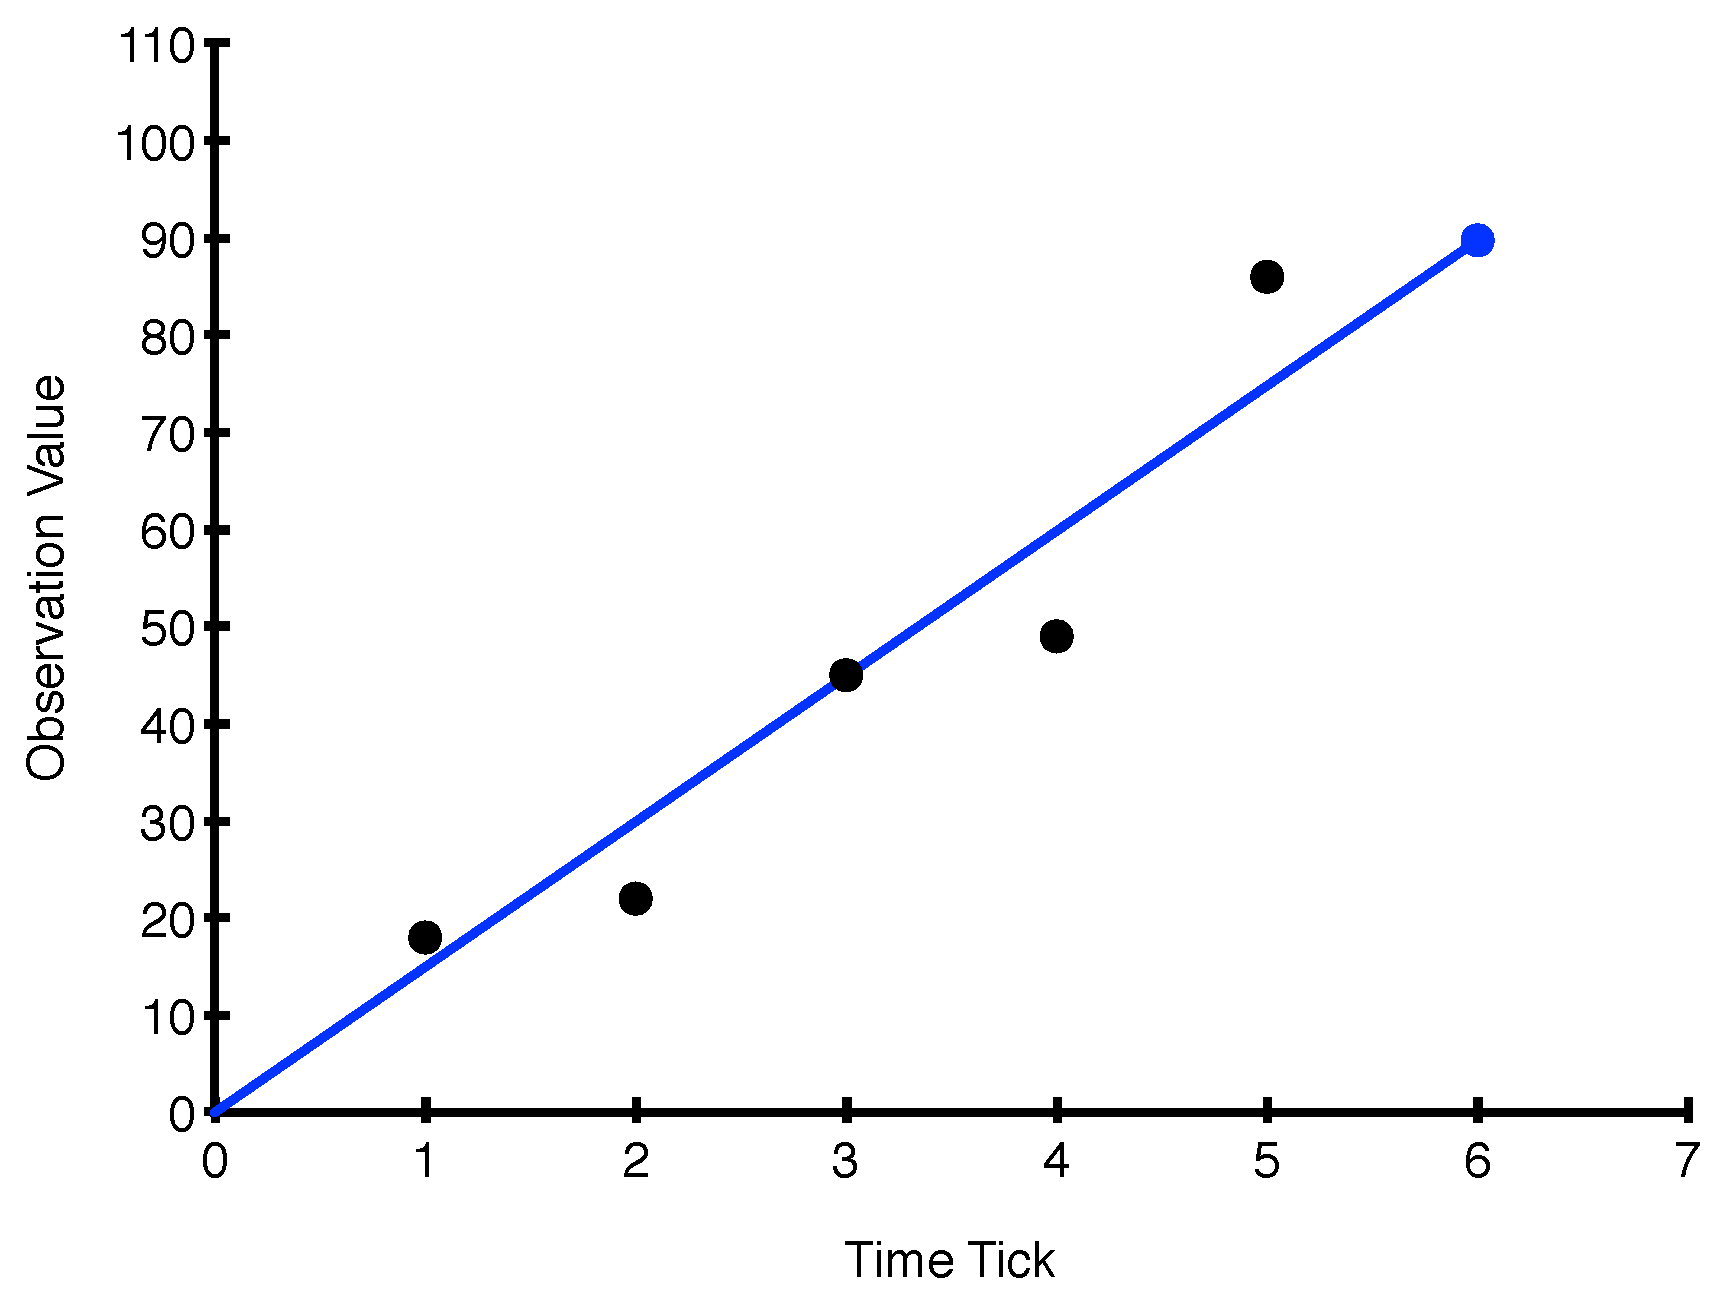
\includegraphics[width=1\textwidth]{lectModel2/LSReg1Line6.pdf}\\
\end{column}
\end{columns}

\end{frame}

%***********************************************************
\begin{frame}{Advantages and Disadvantages of Least Squares}
\begin{itemize}
\item[?]
\end{itemize}
\end{frame}

%***********************************************************
\begin{frame}{Advantages and Disadvantages of Least Squares}
\begin{itemize}
\item Advantages
\begin{itemize}
\item Penalizes values as our predictions move further and further away from the observations
\item Mathematical convenience
\end{itemize}
\item Disadvantages
\begin{itemize}
\item Very sensitive to outliers
\item May require pre-processing / ``cleaning'' before it can be used
\end{itemize}
\end{itemize}
\end{frame}

%***********************************************************
\begin{frame}{Other Loss Functions}

\begin{itemize}

\item View the list of prediction errors $\left(f(t_i) - x_i \right)$ as a vector
\item Can have many loss functions, corresponding to norms
\item Given a vector of errors $\langle \epsilon_1, \epsilon_2, ..., \epsilon_n \rangle$,
$l_p$ norm defined as:
$$||l||_p = \left(\sum_{i = 1}^n |\epsilon_i|^p \right)^{1/p}$$
\item Norm maps a vector to a non-negative scalar
\item Reflect different ``distance'' measures
\end{itemize}
\end{frame}
%***********************************************************
\begin{frame}{Other Loss Functions}

\begin{itemize}
\item Common loss functions correspond to various norms:
\begin{enumerate}
	\item $l_1$ corresponds to mean absolute error. This is taxi cab or Manhattan norm
	\begin{itemize}
	\item Used in LASSO
	\end{itemize}

%	\item[] $||l||_1 = \sum_i |f(t_i) - x_i|$
%	\begin{itemize}
%	\item Also known as ``taxicab'' or ``Manhattan'' norm
%	\item Right angle distance between two locations
%	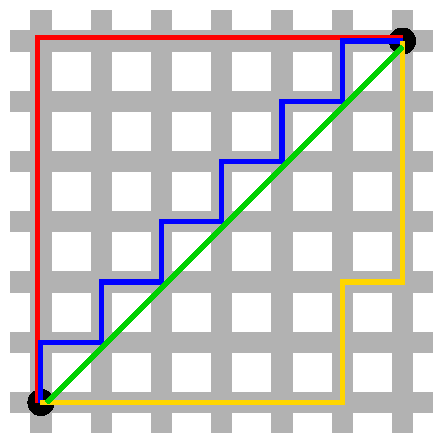
\includegraphics[width=.25\textwidth]{lectModel2/Manhattan_distance.pdf}\\ %https://upload.wikimedia.org/wikipedia/commons/0/08/Manhattan_distance.svg
%	\end{itemize}
	\item $l_2$ to mean squared error/least squares. This is the Euclidean norm
	\item $l_{\infty}$ to the max absolute value. This is the Maximum norm
	\item $l_0$ to the number of non-zero values. This is the Zero norm
\end{enumerate}
\end{itemize}
\end{frame}
%***********************************************************

\begin{frame}{How to Choose a Norm}

\begin{itemize}
\item Zero norm is difficult to optimize since it is discrete
\item Taxicab, Euclidean, and Maximum norms are all convex
\item Euclidean norm is differentiable everywhere. This is a very useful property

\end{itemize}
\end{frame}
%***********************************************************
\begin{frame}{Approaches to Learning a Model}

\begin{itemize}
\item There are many, including:
\begin{enumerate}
\item Optimization based (Least Squares)
\item Probabilistic: MLE (Maximum Likelihood Estimation)
\item Probabilistic: Bayesian
\item Deep Learning
\end{enumerate}
%\item We will cover the first 3
\end{itemize}
\end{frame}
%***********************************************************

\begin{frame}{Maximum Likelihood}

\begin{itemize}
\item Often we have a proper stochastic model
% what is a stochastic model? A Random process that produces data
\item Ex: observed $\{18, 22, 45, 49, 86\}$ (same as before)
\item Model is Exponential, unknown $\lambda$
\item How to estimate? 
\begin{itemize}
\item Most commonly: perform MLE
\item Ignoring time ticks (for now)
\end{itemize}
\item You choose the parameters to maximize the likelihood of getting the observed data
\end{itemize}
\end{frame}
%***********************************************************

\begin{frame}{Likelihood}

\begin{itemize}
\item First, need the notion of a ``likelihood function''
\item Best illustrated with an example
\begin{itemize}
\item In our case, $f (x_i | \lambda) = \lambda e^{-\lambda x_i}$
\item Recall that $f (x_i | \lambda)$ is the probability density of the $i$th point
\item So $f(x_1, x_2, ..., x_n | \lambda) = \prod_i \lambda e^{-\lambda x_i}$ 
\item Assume iid, so the density is a product. % add slide on iid
\item This is a PDF
\end{itemize}
\end{itemize}
\end{frame}
%***********************************************************

\begin{frame}{Likelihood}

\begin{itemize}
\item A ``likelihood function'' simply turns the parametrization around
\begin{itemize}
\item Instead of  $f (x_i | \lambda)$, we have  $f (\lambda | x_i )$
\item So $L (\lambda | x_1, x_2, ..., x_n) = \prod_i \lambda e^{-\lambda x_i}$
\item Now $L$ measures the goodness of the parameter $\lambda$
\item And NOT how likely $x_1, x_2, ..., x_n$ are given the model
\end{itemize}
\end{itemize}
\end{frame}
%***********************************************************
\begin{frame}{Maximum Likelihood Estimation - MLE}

\begin{itemize}
\item Given $L(\Theta \footnote{$\Theta$ is commonly used to denote a set of parameters} | D)$ ($\Theta$ is set of model params, $D$ is data)...
	\begin{itemize}
	\item The MLE $\hat{\Theta}$ for $\Theta$ is defined as the value such that
		$$\forall \hat{\Theta'}, \textrm{ } L(\hat{\Theta'} | D) \leq L(\hat{\Theta} | D)$$
	\item In other words: $\hat{\Theta}$ is the best possible set of parameters, given the available data
	\item Note: closely related to least squares, for normally distributed data
	\end{itemize}
\item[?] Why do we like it?
\end{itemize}
\end{frame}
%***********************************************************
\begin{frame}{MLE}

\begin{itemize}
\item Given $L(\Theta | D)$ ($\Theta$ is set of model params, $D$ is data)...
	\begin{itemize}
	\item The MLE $\hat{\Theta}$ for $\Theta$ is defined as the value such that
		$$\forall \hat{\Theta'}, \textrm{ } L(\hat{\Theta'} | D) \leq L(\hat{\Theta} | D)$$
	\item Note: closely related to least squares!!
	\end{itemize}
\item Why do we like it?
	\begin{itemize}
	\item Under many conditions, it is the Minimum-variance unbiased estimator (``MVUE'')
	\item Under many conditions, error is asymptotically normal
	\item This allows us to talk about confidence bounds
	\end{itemize}
\end{itemize}
\end{frame}

%***********************************************************
\begin{frame}{Minor Digression: Sources of Error}

\begin{itemize}
\item Two most concerning ones
\item Bias
	\begin{itemize}
	\item ``Expected error''
	\item How far off your are on Expectation
	\item e.g. Guess a number, many times
	\item If my average error is +2, this is an example of bias
	\end{itemize}
\item Variance
	\begin{itemize}
	\item ``Spread''
	\item How far from correct your mean guess is
	\end{itemize}
\end{itemize}
\end{frame}
%***********************************************************
\begin{frame}{MLE Example}

\begin{itemize}
\item Want to find the decay parameter in an exponential distribution
\item Might start with an unbiased estimator with low variance
\item Classic estimators are often unbiased, due to asymptotic properties
\item Are these the best to use?
\begin{itemize}
\item Often not
\item However, they are easy to use 
\item And produce reasonable results
\end{itemize}
\end{itemize}

\end{frame}

%***********************************************************
\begin{frame}{Example MLE}

\begin{itemize}
\item Ex: observed $\{18, 22, 45, 49, 86\}$
\item Assume iid, so take the product of the likihoods
\begin{itemize}
\item $L (\lambda | x_1, x_2, ..., x_n) = \prod_i \lambda e^{-\lambda x_i}$
\item Typically, we maximize the log likelihood (LLH) instead:
	$$ \log \Big( \prod_i \lambda e^{-\lambda x_i}\Big) = \sum_i \log (\lambda e^{-\lambda x_i}) =  \sum_i \log (\lambda) + \log ( e^{-\lambda x_i}) = \sum_i  \Big(\log (\lambda)  -\lambda x_i \Big)$$\\
% old formula:	$$\sum_i \Big(-\lambda x_i + \log (\lambda) \Big)$$ \\
% how to get there:
%	$ \sum_i \log (\lambda e^{-\lambda x_i}) =\sum_i\Big( \log ( e^{-\lambda x_i}) +  \log(\lambda) )\Big)$\\
%	$ =    \sum_i \Big(-\lambda x_i + \log(\lambda)\Big)$
\item Again, this is convex:
\begin{align}
L'(\lambda) &=  \sum_i \Big(  \lambda^{-1} -x_i \Big) \nonumber \\
	    &=   5 \lambda^{-1} -220   \nonumber 
\end{align}
\end{itemize}
\end{itemize}
\end{frame}

%***********************************************************
\begin{frame}{Why $\log$?}

\begin{itemize}
\item The math is easier
\item It turns products into sums 
\begin{itemize}
\item Handy for functions of the form $e^{something}$
\end{itemize}
\item It handles really small numbers well
\item The ordering of doesn't change
\begin{itemize}
\item If we have $f(x)$ and we choose an $x$ that maximizes $f$
\item The same $x$ will maximize $\log(f(x))$
\end{itemize}
\end{itemize}
\end{frame}

%***********************************************************
\begin{frame}{Example MLE}

\begin{itemize}
\item Setting the derivative equal to zero,
\begin{align}
0 &= 5 \lambda^{-1} -220   \nonumber \\
\frac{220}{5} &= \lambda^{-1} \nonumber \\
\lambda &= \frac{5}{220} = 0.0227 \nonumber 
\end{align}
\end{itemize}

\end{frame}
%***********************************************************

\begin{frame}{More Complicated MLE}

\begin{itemize}
\item Recall from last lecture, we want to predict how many students will turn in their assignments at least 1 hour before the deadline
\item $\{18, 22, 45, 49, 86\}$ are the known assignment completion times
\item Only 5/10 finished at time 100
\item We did this before, right?
\item What's a problem we ignored last time?
	\begin{itemize}
	\item 5 people not done, but they contribute information
	\item[?] How to model?
	\end{itemize}
\end{itemize}

\end{frame}
%***********************************************************

\begin{frame}{More Complicated MLE}

\begin{itemize}
\item $\{18, 22, 45, 49, 86\}$ are the known assignment completion times
\item Only 5/10 finished at time 100
\item What's a problem with the last model?
	\begin{itemize}
	\item 5 people not done, but they contribute information
	\item How to model?
	\end{itemize}
\item Recall that the exponential distribution is good for modeling arrival times
\item It's also has a really nice CDF: $1- e^{-\lambda x}$
\item Each of 5 who have not yet submitted have $x_i \geq 100$
	\begin{itemize}
	\item So for $i \geq 6$, Pr$[\textrm{no submission}] = 1 - (1 - e^{-\lambda 100})$
	\item Now, $L (\lambda | x_1, x_2, ..., x_n) = \prod_{i = 1}^5 ( \lambda e^{-\lambda x_i}) \times
			\prod_{i = 6}^{10} e^{-\lambda 100}$
	\item[?] Where does the first term come from? % PDF for first 5 students, since we know when they turned in the assignment
	\end{itemize}
\end{itemize}
\end{frame}
%***********************************************************

\begin{frame}{More Complicated MLE}

\begin{itemize}
\item $\{18, 22, 45, 49, 86\}$ are the known assignment completion times
\item Only 5/10 finished at time 100
\item What's a problem with the last model?
	\begin{itemize}
	\item 5 people not done, but they contribute information
	\item How to model?
	\end{itemize}
\item Recall that the exponential distribution is good for modeling arrival times
\item It's also has a really nice CDF: $1- e^{-\lambda x}$
\item Each of 5 who have not yet submitted have $x_i \geq 100$
	\begin{itemize}
	\item So for $i \geq 6$, Pr$[\textrm{no submission}] = 1 - (1 - e^{-\lambda 100})$
	\item Now, $L (\lambda | x_1, x_2, ..., x_n) = \prod_{i = 1}^5 ( \lambda e^{-\lambda x_i}) \times
			\prod_{i = 6}^{10} e^{-\lambda 100}$
	\item Where does the first term come from? 
	\item	 PDF for first 5 students, since we know when they turned in the assignment
	\end{itemize}
\end{itemize}
\end{frame}
%***********************************************************

\begin{frame}{More Complicated MLE}


\begin{itemize}
\item Ex: observed $\{18, 22, 45, 49, 86\}$
\item $L(\lambda | .) = \prod_{i = 1}^5 \lambda e^{-\lambda x_i} \times \prod_{i = 6}^{10} e^{-\lambda 100}$
\item LLH instead: $L(\lambda | .) = \sum_{i = 1}^5 \Big(-\lambda x_i + \log (\lambda) \Big)+
		\sum_{i = 6}^{10} -\lambda 100$
\begin{itemize}
	\item Now, minimizing:
	\begin{align}
		L'(\lambda) &= \sum_{i = 1}^5 \Big( -x_i + \frac{1}{\lambda}\Big) - \sum_{i = 6}^{10} 100 \nonumber \\
			&=  \sum_{i = 1}^5 \Big(-x_i + \frac{1}{\lambda}\Big) - 500 	\nonumber \\
			& = -220 + \frac{5}{\lambda} - 500	\nonumber \\
			&= \frac{5}{\lambda} - 720 \nonumber
	\end{align}
\end{itemize}
\end{itemize}
\end{frame}
%***********************************************************

\begin{frame}{More Complicated MLE}

\begin{itemize}
	\item Setting to zero, we have
	\begin{align} 
			0 &= \frac{5}{\lambda} - 720 \nonumber \\
		 	720 &= \frac{5}{\lambda}  \nonumber \\
			\lambda &= \frac{5}{720} \nonumber
	\end{align}
	\item This is $0.00694$
	\begin{itemize}
	\item So now, probability that a given person (who hasn't turned in) submits within the next 67 hours is $0.372$
	\item $Pr[\textrm{submission}] = 1 - e^{-\lambda x} =1 -* e^{-0.0064 * 167} = 0.372$
	\item Before, it was $0.781$
	\end{itemize}
\end{itemize}
	\end{frame}
%***********************************************************

\begin{frame}{Interpreting the Results}
\begin{itemize}
	\item Before, we were more certain that someone who hadn't submitted the assignment would
	\item Now we are less certain
	\item The probability has dropped about in half 
	% more weight in tail??? 
	% add diagram?
	
\end{itemize}

\end{frame}

%***********************************************************
\begin{frame}{Approaches to Learning a Model}

\begin{itemize}
\item There are many, including:
\begin{enumerate}
\item Optimization based (Least Squares)
\item Probabilistic: MLE (Maximum Likelihood Estimation)
\item Probabilistic: Bayesian
\item Deep Learning
\end{enumerate}
%\item We will cover the first 3
\end{itemize}
\end{frame}
%***********************************************************

\begin{frame}{Bayesian}

\begin{itemize}
	\item Complaint regarding MLE approach:
	\item ``It assumes zero knowledge about the parameter(s) you are trying to estimate''
	\item Do we ever have zero knowledge?
	\item Bayesians say we always know something
	\begin{itemize}
		\item Scores so far: $\{99, 92, 94, 94, 88\}$
		\item Is the mean best estimated as $(99 + 92 + 94 + 94 + 88) / 5$?
		\item Not according to a Bayesian
		\item What if I'd never given an assignment with an average > 90 in my career?
	\end{itemize}
\end{itemize}
	\end{frame}
%***********************************************************

\begin{frame}{Goin' Bayesian}

\begin{itemize}
	\item To a Bayesian:
	\begin{itemize}
		\item ``Learning'' is all about updating one's prior opinions in response to evidence
		\item It's not about guessing parameters
	\end{itemize}
	\item ``Prior opinions'' formally given in the form of a ``prior distribution''
	\begin{itemize}
		\item Pretend I'm a really tough professor
		\item The average score on assignments is around 50
		\item Highest ever was 65
		\item Lowest ever was 35
		\item So I choose Normal$(50, 25)$ as the ``prior'' on the mean assignment score, $\mu$
		\item Why variance of 25?
		\begin{itemize}
		\item Here, 50 is mean, 5 is standard deviation
		\item Standard deviation of 5 chosen as 99.7\% of mass of Normal is $\pm3$ std. devs. from mean
		\item $50 \pm 5$ just covers lowest ever, highest ever
		\end{itemize}
	\end{itemize}
\end{itemize}
\end{frame}
%***********************************************************

\begin{frame}{Bayes' Rule}

\begin{itemize}
	\item A Bayesian uses data $X$ to update the prior on the parameter set $\Theta$
	\begin{itemize}
		\item Resulting distribution---$P(\Theta|X)$ is called the ``posterior''
	\end{itemize}
	\item Update is accomplished via ``Bayes' Rule''
	$$P(\Theta | X) = \frac{P(\Theta) P(X | \Theta)}{P(X)}$$
	$$P(\Theta | X) =  \frac{\textrm{Prior on\ }\Theta \times \textrm{Likelihood}}{\textrm{Normalizing constant}} $$
	\item Can usually drop $P(X)$ as a constant, so we have
	$$P(\Theta | X) \propto P(\Theta) P(X | \Theta)$$
\end{itemize}
\end{frame}
%***********************************************************

\begin{frame}{Notes on Bayes' Rule}

\begin{itemize}
	\item[?] Why can we drop P(X)?
	\begin{itemize}
		\item We are asking: What is the posterior distribution, given \textbf{fixed} data?
		\item Since the data are fixed (observed), P(X) doesn't change the relative ordering
	\end{itemize}
	\item Change the notation to $\propto$ since there is some constant needed for equality
	\item P(X) is usually very difficult to compute
	\item Must integrate over all possible values of the parameters
	$$P(X) = \int P(X|\Theta)$$
\end{itemize}
\end{frame}
%***********************************************************

\begin{frame}{Bayes' Rule Example}

\begin{itemize}
	\item Scores so far: $\{99, 92, 94, 94, 88\}$
	\begin{itemize}
	\item Mean score $\mu \sim \textrm{Normal}(50, 25)$
	\item Each score $x_i \sim \textrm{Normal}(\mu, 16)$
	\item Note: 16 chosen arbitrarily (in practice, maybe this is the historical per-score standard deviation)
	\item Could also replace 16 with a prior (but don't here, for simplicity)
	\item Applying Bayes' rule:
		$$P(\mu | \textrm{data}) \propto \textrm{Normal}(\mu|50, 25) \prod_i \textrm{Normal}(x_i|\mu, 16)$$
	\item Note: this is a function of 1 variable!
	\end{itemize}
\end{itemize}
\end{frame}
%***********************************************************

\begin{frame}{Bayes' Rule Example}
\begin{columns}[T]
\begin{column}{0.7\textwidth}
	$P(\mu | \textrm{data})$
	\begin{align}
	&\propto \textrm{Normal}(\mu|50, 25) \prod_i \textrm{Normal}(x_i|\mu, 4) \nonumber \\
	% plug in distributions
		%%&= \frac{1}{\sqrt{2\pi \times 25}} e^{-\frac{(\mu-50)^2}{2\times 25}} \prod_i \frac{1}{\sqrt{2\pi \times 16}}e^{-\frac{(\mu - x_i)^2}{2\times 16}}  \nonumber \\
		&= 5^{-1} (2\pi)^{-\frac{1}{2}}
                e^{-\frac{1}{2}(\mu - 50)^2 5^{-2}} \prod_i 4^{-1} (2\pi)^{-\frac{1}{2}}
                e^{-\frac{1}{2}(\mu - x_i)^2 4^{-2}}  \\
		% drop constants
%%		& \propto e^{-\frac{(\mu - 50)^2}{2 \times 25}}  \prod_i e^{-\frac{(\mu - x_i)^2}{2 \times 16}}\nonumber \\
		&\propto e^{-\frac{1}{2}(\mu - 50)^2 5^{-2}} \prod_i e^{-\frac{1}{2}(\mu - x_i)^2 4^{-2}}  \\
		% product of e^ = sum of
%%		& \propto e^{-\frac{(\mu - 50)^2}{2 \times 25}}  \sum_i {\frac{(\mu - x_i)^2}{16}}\nonumber \\
		&= e^{-\frac{1}{2} \left( (\mu - 50)^2 5^{-2} + \sum_i (\mu - x_i)^2 4^{-2} \right)}  \\
		&= e^{-\frac{1}{2} \left( 5^{-2} \mu^2 - 100 \times 5^{-2} \mu + 2500 \times 5^{-2} +
			\sum_i 4^{-2} \mu^2 - 2 \times 4^{-2} \mu x_i + 4^{-2} x_i^2 \right)}  
	\end{align}
\end{column}
\begin{column}{0.3\textwidth}
\begin{enumerate}
\vspace{4.3em}
\item Plug in distributions
\vspace{1em}
\item Drop constants % anything that is not a function of \mu is a constant
\vspace{1em}
\item Apply exponent product rule %Product of exponents = $e^{sum of exponents}$ e^m e^n = e^(m+n)
\vspace{.5em}
\item Expand
\end{enumerate}
\end{column}
\end{columns}
%	Come up for air...
	
%	BTW: what's the deal with $\propto$?
%
%	\begin{itemize}
%		\item In the Bayesian world, we are interested in a particular variable ($\mu$ in our case)
%		\item Any time we have $\mu \times (\textrm{value not depending on } \mu)$...
%	\begin{itemize}
%		\item Just drop the value. Justification?
%		\item This is only a normalizting constant
%		\item Required to make distribution integrate to 1
%		\item But useless for comparing goodness of different $\mu$
%	\end{itemize}
%	\end{itemize}
\end{frame}
%***********************************************************

\begin{frame}{Bayes' Rule Example}

\begin{columns}[T]
\begin{column}{0.7\textwidth}
	More math...
	\begin{align}
		&= e^{-\frac{1}{2} \left( 5^{-2} \mu^2 - 100 \times 5^{-2} \mu + 2500 \times 5^{-2} +
			\sum_i 4^{-2} \mu^2 - 2 \times 4^{-2} \mu x_i + 4^{-2} x_i^2 \right)}  \\
		&\propto e^{-\frac{1}{2} \left( 5^{-2} \mu^2 - 4 \mu + \sum_i 4^{-2} \mu^2 - 2 \times 4^{-2} 
			\mu x_i \right)}  \\
		&= e^{\left( 2 + \frac{1}{16} \sum_i x_i \right) \mu - \left( \frac{1}{50} + \frac{5}{32} 
			\right) \mu^2}  \\
		&= e^{a \mu^2 + b \mu} \textrm{ where } a = -\frac{1}{50} -\frac{5}{32}, 
			b = 2 + \frac{1}{16} \sum_i x_i 
	\end{align}
\end{column}
\begin{column}{0.3\textwidth}
\begin{enumerate}
\setcounter{enumi}{4}
\vspace{1.6em}
\item From the last slide
\vspace{.5em}
\item Simplify \& drop constant terms
%\vspace{.5em}
\item Do some more math
\item Apply exponential quadratic function
\end{enumerate}
\end{column}
\end{columns}

	Now things look relatively simple...
\end{frame}
%***********************************************************

\begin{frame}{Bayes' Rule Example}
\begin{itemize} 
	\item We have $P(\mu | \textrm{data}) \propto e^{a \mu^2 + b \mu}$, where:
	\item $a = -\frac{1}{50} -\frac{5}{32} = -0.17625$
	\item $b = 2 + \frac{1}{16} \sum_i x_i = 31.1875$
	\begin{itemize}
		\item By definition, this is $\propto \textrm{Normal}(-b/(2a), -1/(2a))$
		\item Plug in our data to get values for $a$ and $b$
		\item Or, $\textrm{Normal}(88.475, 2.89)$
	\end{itemize}
	\item Recall: Questioning if the mean was best estimated as $(99 + 92 + 94 + 94 + 88) / 5 = 93.4$
	\item Took into account historical data about scores on assignments 
\end{itemize}
	\end{frame}
%***********************************************************

\begin{frame}{Conjugate Priors}

\begin{itemize} 
	\item That was a LOT of work!!
	\item Easier to use a table of conjugate priors
	\item What is THAT?
	\begin{itemize}
		\item When you have $\Theta \sim f(\theta_{\textrm{prior}})$
		\item And you have $X \sim g(.)$
		\item And you can prove $P(\Theta | X) = f (\Theta | \theta_{\textrm{post}})$
		\item That is, the posterior for $\Theta$ is the same family as the prior
		\item Then we say $f$ is a ``conjugate prior'' for $g$
	\end{itemize}
	\item There are lots of conjugate priors
	\item Key tool in Bayesian's toolbox
	\item Allow us to easily sample new parameter values from a related distribution instead of doing complex math or sampling
\end{itemize}
\end{frame}
%***********************************************************

\begin{frame}{Conjugate Priors}

\begin{itemize} 
%	\item Why useful?
	\item Usually simple rules for computing $\theta_{\textrm{post}}$ 
		from $X, \theta_{\textrm{prior}}$
	\item Search ``Wikipedia conjugate prior''... first result
	\item Find row under ``continuous distributions''
\end{itemize}
				
\end{frame}
%***********************************************************

\begin{frame}{Conjugate Priors}

\begin{itemize} 
		\item When $g(.)$ (likelihood) is Normal with known variance $\sigma_l^2$
		\item $\sigma_l^2 = 16$ in our case
		\item And $f(\theta_{\textrm{prior}})$ is Normal$(\mu_p, \sigma_p^2)$
		\item Observed $n$ data points
		\item Then posterior is easy: In $\theta_{\textrm{post}}$, we have:
		\begin{align}
			\mu &= \frac{\left(\frac{\mu_p}{\sigma^2_p} + \frac{\sum x_i}{\sigma_l^2} \right)}
				{\left(\frac{1}{\sigma^2_p} + \frac{n}{\sigma_l^2} \right) }= 
				\frac{\left( \frac{50}{25} + \frac{467}{16} \right) }{ \left(\frac{1}{25} 
					+ \frac{5}{16}\right)} \nonumber \\
%			\mu &= \left(\frac{\mu_p}{\sigma^2_p} + \frac{\sum x_i}{\sigma_l^2} \right) /
%				\left(\frac{1}{\sigma^2_p} + \frac{n}{\sigma_l^2} \right) = 
%				\left( \frac{50}{25} + \frac{467}{16} \right) / \left(\frac{1}{25} 
%					+ \frac{5}{16}\right) \nonumber \\
			\sigma^2 &= \left(\frac{1}{\sigma^2_p} + \frac{n}{\sigma_l^2} \right)^{-1} =
				\left(\frac{1}{25} + \frac{5}{16}\right)^{-1} \nonumber
		\end{align}
		\item Gives the same result, much less fuss!!
		\item Often drives choice of distribution
\end{itemize}
				
\end{frame}
%***********************************************************
\begin{frame}{Questions?}
\begin{itemize}
	\item[?] How can we use what we learned today?
	\vspace{2em}
	\item[?] What do we know now that we didn't know before?
\end{itemize}
\end{frame}

%***********************************************************
\begin{frame}{Questions?}
\begin{itemize}
	\item[?] How can we use what we learned today?
	\vspace{2em}
	\item[?] What do we know now that we didn't know before?
\begin{itemize}
\item Reviewed 3 different approaches to learn model parameters
\item Learned that the results vary based on 
\begin{itemize}
\item Model used
\item Assumptions
\end{itemize}
\end{itemize}
\end{itemize}
\end{frame}

\end{document}
